\lfoot{Autor: Fitim Faiku}
\subsection{Fahrkomfortanalyse}


Da die bewertung der einzelnen Fahrer durch den Fahrgast erfolgt ist jedem klar.
Diese Bewertung faellt meistens aus den Faktoren wie stark ein Fahrer beschleunigt und in welcher Geschwindigkeit er um eine Kurve faehrt.
Um einen KFZ-Einsteiger mit mueglichst Informativen Daten zu \"bewerten\" habe ich mir einen Kammschen Kreis als Hilfe genommen.

\subsubsection{Kammscher Kreis }
Ein Kammsher Kreis ist ein ein Kreis in dem durch Polarkoordinaten die Extremwerte einer Fahrt eingezeichnet sind.
Der Kreis ist so aufgebaut, dass in Norden de Bremskraefte angezeigt werden, in Süden alle Beschleunigungen, im Westen die Rechtskurven und Osten die Linkskurven.
Es ist also alles verkehrt.
\begin{figure}[!htb]\centering
	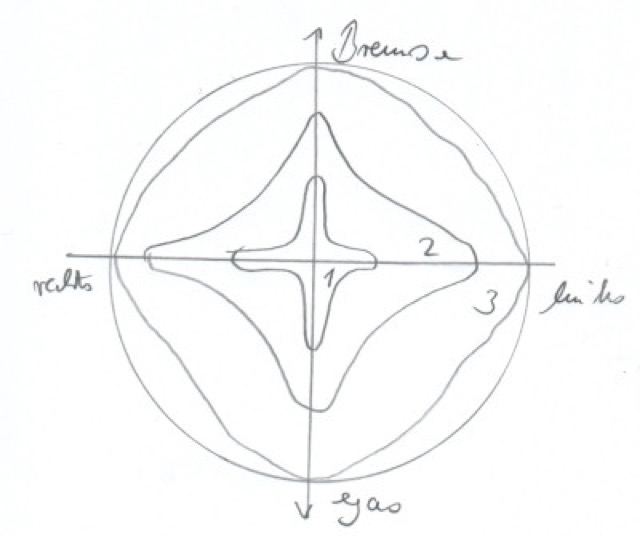
\includegraphics[width=0.5\textwidth]{images/kammsherkreis}
	\caption{Kammsherkreis \cite{FAIF.CH3-fahrkomfortanalyse.KammscherKreis}}\label{Fig:Kammsher-Kreis}
\end{figure}

\subsubsection{Implementierung}
Um diesen Kammschen Kreis richtig darzustellen habe ich mir die Klasse canvas als Hilfe genommen, wobei die von Graphics erbt.
Mittels Canvas konnte ich zufaellig generierte 0-360grad Winkel und Radien erstellen und die dann in Polarkoordinaten umrechnen.
Somit konnte ich alle generierten werte Darstellen. 

\lstinputlisting[caption=Runden-Methode, style=javastyle]{code/Runden.java}

Bei der Methode Runden nehme ich alle Winkel auf und runde sie auf oder ab in 5er Schritten.
\newline 


\lstinputlisting[caption=Draw, style=javastyle]{code/ChartView.java}
Um den Kammshen-Kreis zu zeichnen habe ich die OnDraw Methode ueberschrieben, weiters speichere ich alle generierten Werte in einer Liste welche in einer For-Schleife gezeichnet werden.
\clearpage % DO NOT REMOVE